\begin{figure*}[t]
  \centering
  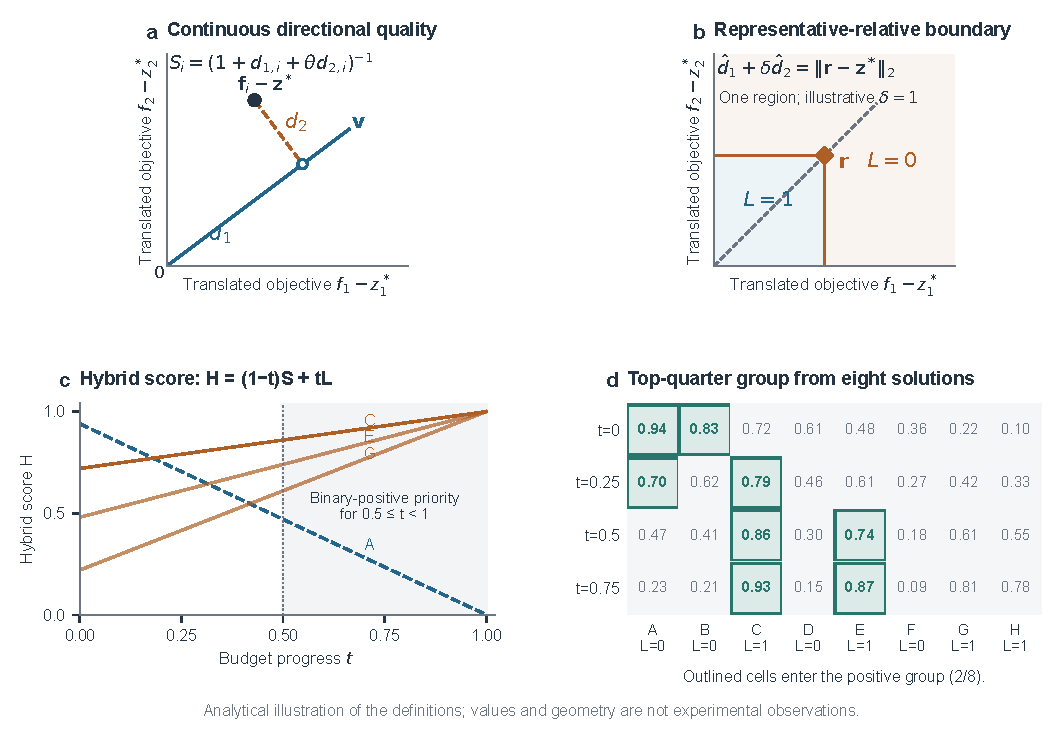
\includegraphics[width=0.98\textwidth]{figures/fig_hybrid_grouping.pdf}
  \caption{Analytical illustration of hybrid PBI grouping.
  (a)~The continuous score decreases with the directional PBI value.
  (b)~A representative defines a relative binary boundary within its associated
  region; this example fixes $\delta=1$, while the implementation adapts $\delta$.
  Panels (a,b) show translated objective coordinates after association.
  (c)~Hybrid-score trajectories for four of the example solutions. Solid curves
  have $L=1$ and the dashed curve has $L=0$; the binary-positive group has
  priority for $0.5\leq t<1$. At $t=1$, scores reduce to the binary labels.
  (d)~Scores of all eight example solutions and the top-quarter positive group
  (outlined cells). The first row lists the example continuous scores $S$;
  the labels $L$ are shown below the columns. The values illustrate
  Eqs.~\eqref{eq:score-cont}--\eqref{eq:group} and are not experimental observations.
  \label{fig:hybrid-grouping}}
\end{figure*}
